Simulations are extremely important for analyzing an application's performance, or more generally, its behavior.
As described in Section~\ref{sec:arch_models}, there are multiple levels of detail in which to model and, consequently, simulate, an architecture and its execution.
For investigating the mapping problem in software synthesis, higher-level simulations are preferable for multiple reasons.
First and foremost, higher-level simulations are faster.
If a meta-heuristic iteratively evaluates dozens, hundreds or even thousands of mappings to find a near-optimal one, it greatly benefits from the fast evaluation time associated with a higher-level simulation.

Higher levels of abstraction come with a trade-off, accuracy of the simulation suffers in exchange for the simpler models and faster simulation times.
Let $\tilde \Theta$ be the approximation of $\Theta$ from the simulation. A loss in accuracy means that $| \Theta(m) - \tilde \Theta(m)|$ becomes larger.
However, depending on the use-case and mapping objective $\Theta$, this loss in simulation accuracy might not necessarily affect the quality software synthesis results.
Suppose that the objective $\Theta$ represents execution time or energy consumption, and the goal of the software synthesis is just a best-effort minimization of $\Theta$ (with no additional constraints, i.e. $C \equiv \operatorname{True}$).
Then the accuracy of the simulation is not important, only its fidelity.
If $\Theta(m_1) < \Theta(m_2)$ we want the result of the simulation to reflect this, $\tilde \Theta(m_1) < \tilde \Theta(m_2)$.
As long as this is the case, we don't care about the actual value of $| \Theta(m_i) - \tilde \Theta(m_i)|$, since in this case the exploration will still find the minimum.
The fidelity of the simulation is a measure of how often this is true.
On the other hand, if the application is a real-time application, then the truth value of $C$ will depend on the accuracy of the simulation.
Here, the accuracy of the simulation is much more important.

This chapter describes the simulation aspects which pertain the models of computation and the practical tooling we will use.
Nuanced simulation details and advanced techniques are beyond the scope of this thesis.

\subsection{Simulating the Execution of Kahn Process Networks}

The behavior of a system plays a central role in simulation. A deterministic model should yield deterministic simulation results.
Non-determinism, when present, should also be captured by the models and reflected by the simulations.

The behavior of systems is commonly captured in execution traces, which simply record the behavior of different entities (e.g. processes or actors) at different timepoints.
This can be formally captured in a monoid structure of (Mazurkiewicz) traces or, equivalently, histories~\cite{diekert1995book}.
Traces are useful to understand the behavior of systems~\cite{vampir} and are common in many domains.
However, for systems that are non-deterministic, (by definition) the behavior of the system does not only depend on the input.
This can make designing~\cite{lee2006problem} and debugging~\cite{murillo_debugging} particularly difficult.
In cyber-physical-sytems or, more generally, reactive systems in the sense of Harel and Pnueli~\cite{harel_pnueli_reactive}, input from the physical world might come in a non-deterministic fashion.
The problem of capturing the behavior of such a system is even more complex when the system is distributed~\cite{shaver_phdthesis}. 

Kahn Process Networks are deterministic, as are all the dataflow models that can be embedded as KPNs.
This means that the behavior of a KPN application depends only on the input to the network.
In particular, it does not on the mapping and scheduling or related execution details.
Thus, their behavior can be captured by a (Mazurkiewicz) trace.
This permits to re-create their behavior in a fashion that is independent of the mapping~\cite{find_proper_references}.
By ``replaying'' the trace, i.e. simulating the execution of a process for every input in the trace, a discrete-event simulator can successfully simulate the execution of a KPN, since the token sequence is guaranteed to be identical given identical inputs.
In particular, this allows us to do design-space exploration.

A discrete-event simulation of a KPN application thus requires behavior traces. It also needs to model the execution and communication times.
Modeling execution times from a trace is simple, with a crucial assumption: if the execution times for a trace event only depend on the PE type.
This assumption won't hold always hold, e.g. when the instruction cache is flushed due to scheduling decisions, or due to unpredictability from the \ac{OS}.
Note that data caches are modeled as part of the communication between processes.
However, in most cases this assumption is a good approximation, it is normal to expect that the same code executing on the same data and the same \ac{ISA} will usually require the same amount of time.

Modeling communication is more complicated, as it depends on the memory subsystem. In general, the communication costs of sending a KPN token depend on multiple factors, like the size of the token, contention in the memory subsystem (and correspondingly methods of arbitration, routing in the case of a \ac{NoC}, etc), or the API and protocol being used.
For the simulations in this thesis, we use a model based on annotations of the architecture graph $A$. These annotations are functions that calculate the time cost of communicating data, as a function of its size.
In this way, we model both the latency and bandwidth of the communication.
We use a split-cost communication model to assign costs to sending and receiving data~\cite{odendahl2013split}.
This separation can be used to simulate based on traces, as described above, since we can then compute the cost of communication for both the sending and receiving processes.

When dealing with \ac{NoC}-based architectures, this model is not as accurate.
Communication over a \ac{NoC} depends also on the routers and links along the path, including the routing algorithms.
We extended the split-cost communication model to account for these issues in~\cite{menard_norcas16}.
The idea is to add a third term to account for the network, in addition to the consumer and producer costs. 
This third term can account for the routing and the topology of the network while maintaining an analytic model which is cheap to evaluate in a high-level simulation.

Simulation is essential for software synthesis, yet it is not the focus of this thesis. As such, we will only discuss the main idea behind the analytic models and their relationship to a fast simulation of \ac{NoC}-based architectures.
The main contribution of~\cite{menard_norcas16}, with a concrete model for the Tomahawk~2 architecture~\cite{tomahawk2} and the corresponding evaluation comparing to the SystemC-based simulator Noxim~\cite{noxim} are due to my coauthors and beyond the scope of this thesis.

\subsection{Mocasin}

In this thesis we will use mocasin, a tool for the Model-of-Computation-based Analysis and Simulation of applications~\cite{menard_rapido21}.
This tool, formerly known as pykpn~\cite{goens_mcsoc18}, has been developed as part of a collaborative effort between multiple researchers at the Chair for Compiler Construction at TU Dresden.
While the tool itself is a joint contribution with the coauthors of~\cite{menard_rapido21}, many concepts introduced in this thesis have been implemented and tested using mocasin.
As such, this section will explain the tool in-depth, to enable the description of the different implementations of contributions from this thesis implemented in mocasin.

\begin{figure}[h]
	\centering
   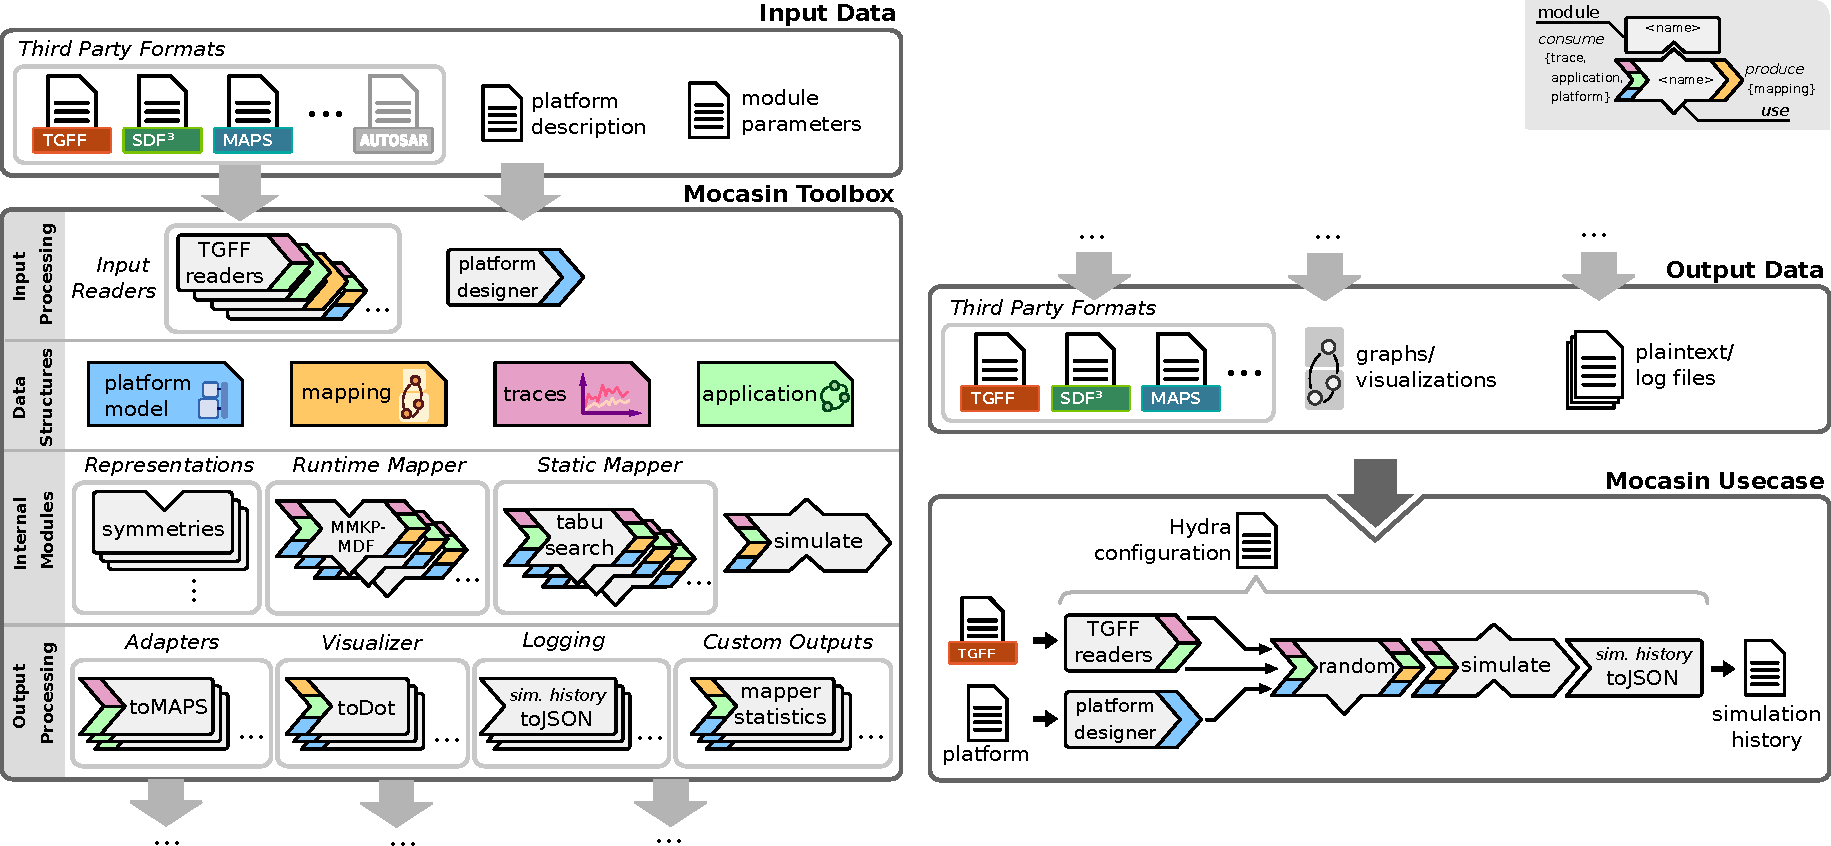
\includegraphics[width=0.5\textwidth]{figures/mocasin.pdf}
	\caption{The mocasin architecture. Repreinted from \cite{menard_rapido21} (Figure~2).}
	\label{fig:mocasin_kpn_simulation}
\end{figure}


Figure~\ref{fig:mocasin_kpn_simulation} depicts the basic flow of simulating KPN applications in mocasin.
In general, simulating a KPN requires four inputs, as explained in Section~\ref{sec:mappings_background}: the KPN graph, a platform description, execution traces and a mapping.
Instead of a concrete trace, mocasin expects a trace generator, which can generate the trace on the fly: this is useful e.g. for non-deterministic models computation, but for KPNs the two are equvialent.
A mapping, while required for simulation, does not need to be provided: it can be calculated in a design-space exploration.
This is not surprising, since a significant part of Part I of this thesis concerns itself with finding good mappings efficiently.

\subsubsection{simulate}
A central part of mocasin is a discrete-event simulator that uses the principles outlined above to simulate KPN applications based on their traces (as well as other models of computation).


TODO: finish explanation, add figure.

\begin{figure}[h]
	\centering
   \resizebox{0.95\textwidth}{!}{% Define block styles
\tikzstyle{mio} = [rectangle, rounded corners, draw, fill=green!20, %legend: possible "IP leak"
    text width=7em, text centered, minimum height=4em]
\tikzstyle{block} = [rectangle, draw, fill=blue!20, 
    text width=7em, text centered, rounded corners, minimum height=4em]
\tikzstyle{required} = [draw, ->]
\tikzstyle{possible} = [draw, dashed, ->]
\tikzstyle{interaction} = [thick, <->, draw, color=red!70]
\tikzstyle{data} = [rectangle, rounded corners, draw, fill=teal!20, text width=7em, text centered,  minimum height=4em]

\begin{tikzpicture}[node distance = 4em]
    % inputs/readers
    \node [block ] (tgff) {tgff readers};
    \node [block, below=of tgff ] (sdf3) {sdf$^3$ readers};
    \node [block, below=of sdf3] (slx) {SLX readers};

    %data
    \node [data, right=of tgff] (traces) {traces};
    \node [data, below=of traces] (app) {application (e.g. KPN)};
    \node [data, below=of app] (mapping) {mapping};
    \node [data, below=of mapping] (platform) {platform model};

    \node [block, left=of platform] (platformdes) {platform designer};

    %modules
    \node [block, right=of mapping] (mappers) {mappers};
    \node [block, right=of app] (simulate) {simulate};
    \node [mio, above=of simulate] (tetris) {runtime managers (Section~\ref{sec:tetris}) };
    \node [mio, right=of mappers] (logic) {logic language manager (Section~\ref{sec:logic_language})};
    \node [mio, below=of mappers] (representations) {representations (Chapter~\ref{chap:mapping_structures})};
    \node [mio, above=of logic, align=center] (dc) {design centering \\ (Section~\ref{sec:design_centering})};


    %edges
    \path [possible] (slx) -- (traces);
    \path [possible] (slx) -- (app);
    \path [possible] (slx) -- (platform);
    \path [possible] (slx) -- (mapping);

    \path [possible] (tgff) -- (traces);
    \path [possible] (tgff) -- (app);
    \path [possible] (sdf3) -- (traces);
    \path [possible] (sdf3) -- (app);

    \path [possible] (platformdes) -- (platform);

    \path [required] (traces) -- (mappers);
    \path [required] (app) -- (mappers);
    \path [required] (platform) -- (mappers);
    \path [required] (mappers) -- (mapping);



    \path [required] (traces) -- (simulate);
    \path [required] (app) -- (simulate);
    \path [required] (platform) -- (simulate);
    \path [required] (mapping) -- (simulate);

    %interactions
    \path [interaction] (mappers) -- (logic);
    \path [interaction] (mappers) -- (representations);
    \path [interaction] (simulate) -- (tetris);
    \path [interaction] (simulate) -- (mappers);
    \path [interaction] (simulate) -- (dc);

    \matrix [draw=black,fill=gray!10,above=13em of traces.north west, anchor=north west] {
      \node[data, rounded corners=0, text width=1em, minimum height=1em] {}; & \node[] {data structure};\\
      \node[block, rounded corners=0, text width=1em, minimum height=1em] {}; & \node[] {module};\\
      \node[mio, rounded corners=0, text width=1em, minimum height=1em] {}; & \node[] {module with contributions from this thesis};\\
      \draw[possible] (0,-0.2) -- (0.4,-0.2); & \node[] {optional input data};\\
      \draw[required] (0,-0.2) -- (0.4,-0.2); & \node[] {internal data depencency};\\
      \draw[interaction] (0,-0.2) -- (0.4,-0.2); & \node[] {interaction between modules};\\
      % \node[fill=black,draw,circle,inner sep=2pt,outer sep=0pt] (m) at (0,0){};
      % \draw (m) -- +(0,0.4); & \node[legendtext]{Mandatory}; & 
 %   \filldraw[fill=white,draw=black] (0,0.2) -- ++(225:0.2) arc[start angle=225,end angle=315,radius=0.2]; 
 % \draw (0,0.2) ++(225:0.5) -- (0,0.2) -- ++(315:0.5);& \node[legendtext]{Alternative}; \\
 %  \node[fill=white,draw=black,circle,inner sep=2pt,outer sep=0pt] (o) at (0,0){}; \draw (m) -- +(0,0.4); & \node[legendtext]{Optional}; & 
 %  \draw (0,0.2) ++(225:0.5) -- (0,0.2) -- ++(315:0.5);
 %  \filldraw[black] (0,0.2) -- ++(225:0.2) arc[start angle=225,end angle=315,radius=0.2]; & \node[legendtext]{Or}; 
\\
};
\end{tikzpicture}
}
	\caption{Simulating KPN Applications in mocasin. TODO: this figure should actually come later}
	\label{fig:mocasin_kpn_simulation}
\end{figure}
